\setcounter{chapter}{3}
\chapter{Propriétés générales des niveaux électroniques dans un 
potentiel périodique}
Dans un cristal, les ions sont disposés de façon périodique, il faut 
considérer le problème d'un électron dans un potentiel périodique 
avec la périodicité du réseau de Bravais :
\begin{equation}
U(\vec{r}+\vec{R}) = U(\vec{r})\qquad\forall\vec{R} \in \text{réseau 
de Bravais}
\end{equation}
Ceci offre une symétrie de translation, mais uniquement discrètes 
sinon le potentiel serait constant et la solution de l'équation 
de Schrödinger serait des ondes planes. Cette périodicité étant proche de 
la longueur d'onde des électrons, il faut faire intervenir la physique 
quantique. Hélas, à part ce document, rien n'est parfait : la 
périodicité parfaite n'existe pas. On procédera en deux étapes :
\begin{enumerate}
\item On travaille le cas parfaitement périodique.
\item On traite les dérivation de la périodicité parfaite comme des 
perturbations.
\end{enumerate}

	\section{Le potentiel périodique}
	\begin{wrapfigure}[10]{l}{7.5cm}
	\vspace{-0.5cm}
	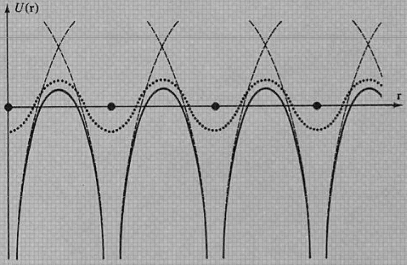
\includegraphics[scale=0.5]{ch4/image1.png}
	\captionof{figure}{ }
	\end{wrapfigure}
	Si le cristal est périodique, le potentiel vu par les électrons 
	le sera également. Un tel potentiel est représenté ci-contre : 
	il ressemble à des potentiels individuels atomiques. On étudiera 
	ainsi les propriétés de l'équation de Schrödinger d'un électron 
	\begin{equation}
	H\psi = \left\{-\frac{\hbar^2}{2m}\Delta + U(\vec{r})\right\}\psi 
	= \varepsilon\psi
	\label{eq:Schod}
	\end{equation}
	avec $U(\vec{r})$ périodique. Si $U(\vec{r})=0$, on retrouve le 
	modèle de Sommerfeld.
	
	\section{Théorème de Bloch}
	\theor{\textsc{Bloch}\\
	Les vecteurs propres $\psi$ de l'opérateur hamiltonien à un 
	électron $H = -(\hbar^2/2m)\Delta + U(\vec{r})$ où $U(\vec{r} +
	\vec{R})=U(\vec{r})\ \ \forall \vec{R}\in\text{ au réseau de 
	Bravais}$ ont la forme d'une onde plane multipliée par une 
	fonction ayant la périodicité du réseau de Bravais :
	\begin{equation}
	\psi_{n\vec{k}}(\vec{r}) = e^{i\vec{k}\vec{r}}u_{n\vec{k}}(\vec{r
	})
	\end{equation}
	où $u_{n\vec{k}}(\vec{r}+\vec{R}) = u_{n\vec{k}}(\vec{r})$. Notons
	que (remplacer $\vec{r}$ par $\vec{r}+\vec{R}$, le résultat 
	est immédiat) :
	\begin{equation}
	\psi_{n\vec{k}}(\vec{r}+\vec{R}) = e^{i\vec{k}\vec{R}}\psi_{n\vec{k}}
	(\vec{r})
	\end{equation}	}\ \\
	Une formulation alternative est : les fonctions propres 
	de $H$ peuvent être choisies de sorte qu'à tout $\psi$ on 
	peut associer un vecteur d'onde $\vec{k}$ tel que 
	\begin{equation}
	\psi(\vec{r}+\vec{R}) = e^{i\vec{k}\vec{R}}\psi(\vec{r})
	\end{equation}
	$\forall\vec{R} \in$ au réseau de Bravais. Notons que $n$ 
	est l'\textit{indice de bande}.
	
	\section{Première démonstration du théorème de Bloch}
	Pour tout $\vec{R}\in$ réseau de Bravais, on définit un opérateur 
	de translation $T_{\vec{R}}$ qui appliqué donne
	\begin{equation}
	T_{\vec{R}}f(\vec{r}) = f(\vec{r}+\vec{R})
	\end{equation}
	Cet opérateur permute avec $H$, qui est périodique 
	\begin{equation}
	T_{\vec{R}}H\psi = H(\vec{r}+\vec {R})\psi(\vec r+\vec R) = H(\vec{r})
	\psi(\vec r+\vec R) = HT_{\vec{R}}\psi \Longrightarrow[H,T_{\vec{R}}]=0
	\end{equation}
	On aura donc une base de fonction propres commune : 
	$\left\{\begin{array}{ll}
	H\psi &= \varepsilon\psi\\
	T_{\vec{R}}\psi &= c(\vec{R})\psi
	\end{array}\right.$. Remarquons le résultat suivant, de deux 
	translations successives :
	\begin{equation}
	T_{\vec{R}}T_{\vec{R'}}\psi(\vec{r})=T_{\vec{R'}}T_{\vec{R'}}\psi(\vec{r})
	=T_{\vec{R+R'}}\psi(\vec{r})
	\end{equation}
	L'ensemble des $T_{\vec{R}}$ commute donc avec $H$ pour tout $\vec{R}$.
	Les valeurs propres $c(\vec{R})$ sont ainsi lié à cet opérateur : 
	\begin{equation}
	\left.\begin{array}{lll}
	T_{\vec{R'}}T_{\vec{R}}\psi &= c(\vec{R'})T_{\vec{R}}\psi &= c(\vec{R'})
	c(\vec{R})\psi\\
	T_{\vec{R'}}T_{\vec{R}}\psi &=T_{\vec{R'}+\vec{R}}\psi &=c(\vec{R'}+
	\vec{R})\psi
	\end{array}\right\}\Rightarrow c(\vec{R})c(\vec{R'}) = c(\vec{R}+\vec{R'})
	\end{equation}
	Les exponentielles répondent à cette égalité. Comme $|\psi|^2$ doit être 
	au maximum unitaire, cet exponentielle doit forcément être imaginaire. On 
	peut donc toujours écrire $c(a_i) = e^{2\pi i x_i}$\footnote{?? Facteur $2\pi?$} \\
	Soit $a_i$, trois vecteurs primitifs du réseau de Bravais tel que 
	$\vec{R} = n_1\vec{a_1}+n_2\vec{a_2}+n_3\vec{a_3}$ et $\vec{k} = x_1\vec{b_1}
	+x_2\vec{b_2}+x_3\vec{b_3}$ où $b_i$ sont les vecteurs primitifs du réseau 
	réciproque. On a alors :
	\begin{equation}
	c(\vec{R}) = c(a_1)^{n_1}.c(a_2)^{n_2}.c(a_3)^{n_3} = e^{i\vec{k}\vec{R}}
	\end{equation}
	Ceci démontre le théorème de Bloch :
	\begin{equation}
	\displaystyle
	T_{\vec{R}}\psi = \psi(\vec{r}+\vec{R}) = c(\vec{R})\psi(\vec{r}) = 
	e^{i\vec{k}\vec{R}}\psi(\vec{r})
	\end{equation}
	$\hfill\square$
	
	\section{Les conditions aux limites de Born - von Karman}
	Il est possible de quantifier $\vec{k}$ en imposant des conditions 
	aux limites stylées, c'est-à-dire la même que pour Sommerfeld sauf 
	que l'on considèrera cette fois un cristal de volume $V$ de forme 
	lié à une cellule primitive du réseau de Bravais :
	\begin{equation}
	\psi(\vec{r}+N_i\vec{a}_i) = \psi(\vec{r})
	\end{equation}
	où les $\vec a_i$ sont les vecteurs primitifs du réseau direct et 
	les $N_i$ des entiers tels que $N = N_1N_2N_3 $ est le nombre de 
	cellules primitives dans le cristal. En appliquant Bloch :
	\begin{equation}
	\displaystyle
	\psi(\vec{r}+ N_i\vec{a_i})_{n\vec k} = e^{i\vec{k}N_i\vec{a_i}}
	\psi_{n\vec k}(\vec{r})= \psi(\vec{r})_{n\vec k} \Longrightarrow 
	e^{i\vec{k}N_i\vec{a_i}} = 1
	\end{equation}
	Inspiré de cette condition et du fait que $\vec{k} = x_1\vec{b_1}
	+x_2\vec{b_2}+x_3\vec{b_3}$, on a\footnote{A éclaircir}
	\begin{equation}
	e^{i2\pi x_iN_i} = 1
	\end{equation}		
	 et on en déduit que $x_1=\frac{m_i}{N_i}$ :
	\begin{equation}
	\vec{k} = \frac{m_1}{N_1}\vec{b_1}+\frac{m_2}{N_2}\vec{b_2}+\frac{m_3}{
	N_3}\vec{b_3} + \dots
	\end{equation}
	On peut voir ceci comme une généralisation des CL de BVK.
	
	
	\section{Seconde démonstration du théorème de Bloch}
	En considérant \autoref{eq:Schod}, on peut toujours développer 
	une fonction $\psi$ satisfaisant les CL de BVK sur l'ensemble 
	des ondes planes satisfaisant ces CL :
	\begin{equation}
	\psi(\vec{r}) = \sum_{\vec{q}} c_{\vec{q}}\ e^{i\vec{q}.\vec{r}}
	\end{equation}
	$U(\vec{r})$ est périodique, il ne contient que des ondes qui 
	ont la périodicité du réseau de Bravais :
	\begin{equation}
	U(\vec{r}) = \sum_{\vec{K}} U_{\vec{K}}\ e^{i\vec{K}.\vec{r}}
	\end{equation}
	où les $U_{\vec{K}}$ sont les coefficients de Fourier du potentiel 
	périodique par association. On pose $U_0=0$, la valeur moyenne 
	du potentiel sur une cellule primitive. Comme $U(\vec{r}) \in 
	\mathbb{R} : U_{-\vec{K}}=U_{\vec{K}}=U_{\vec{K}}^*$ (on suppose 
	également une symétrie d'inversion).\\
	Introduisons nos développement de $\psi$ et $U(\vec{r})$ dans l'
	équation de Schrödinger :
	\begin{equation}
	\frac{p^2}{2m}\psi = -\frac{\hbar^2}{2m}\Delta \psi = \sum_{\vec q}
	\frac{\hbar^2}{2m}q^2c_{\vec{q}}\ e^{i\vec{q}\ \vec{r}} 
	\end{equation}
	On peut écrire le terme de potentiel (en posant $\vec{q'}=\vec{q}+
	\vec{K}$ pour avoir une belle exp.) :
	\begin{equation}
	U\psi = \left(\sum_{\vec{K}}\ e^{i\vec{K}.\vec{r}}\right).\left(
	\sum_{\vec{q}} c_{\vec{q}}\ e^{i\vec{q}.\vec{r}}\right) = \sum_{
	\vec{K}\vec{q}} U_{\vec{K}}.c_{\vec{q}}.e^{i(\vec{K}+\vec{q})\vec{r}}
	= \sum_{\vec{K}\vec{q'}}U_{\vec{K}}\ c_{\vec{q'}-\vec{K}}\ e^{i
	\vec{q'}.\vec{r}}
	\end{equation}
	En posant $\vec{q'}=\vec{q}$, $\vec{K'}=\vec{K}$ (pour avoir des 
	notations similaire au A\&M) et comme $\displaystyle\epsilon\psi = 
	\sum_{\vec{q}} 	\varepsilon\ c_{\vec{q}}\ e^{i\vec{q}.\vec{r}} $, 
	en remettant tout ensemble on obtient\footnote{Ici on ne fait que 
	des math, on n'a fait aucune approximation, juste des remplacements.}
	\begin{equation}
	\sum_{\vec{q}}e^{i\vec{q}.\vec{r}}\left\{\left(\frac{\hbar^2}{2m}q^2
	-\varepsilon\right)c_{\vec{q}} + \sum_{\vec{K'}}U_{\vec{K'}}\ c_{\vec{
	q}-\vec{K'}}\right\}=0
	\end{equation}
	Comme les ondes planes sont orthogonales entre elles, on obtient
	\begin{equation}
	\left(\frac{\hbar^2}{2m}q^2
	-\varepsilon\right)c_{\vec{q}} + \sum_{\vec{K'}}U_{\vec{K'}}\ c_{\vec{
	q}-\vec{K'}}=0
	\end{equation}
	En posant $\vec{q}=\vec{k}-\vec{K}$ où $\vec{K}$ est un vecteur du 
	réseau réciproque et $\vec{k}$ un réseau dans la première zone de 
	Brillouin :
	\begin{equation}
	\left\{\frac{\hbar^2}{2m}|\vec{k}-\vec{K}|-\varepsilon\right\}c_{
	\vec{k}-\vec{K}}+\sum_{\vec{K'}}U_{\vec{K'}}\ c_{\vec{k}-\vec{K}-
	\vec{K'}}=0
	\end{equation}
	En remplaçant $\vec{K'} = \vec{K'}-\vec{K}$ :
	\begin{equation}
	\left\{\frac{\hbar^2}{2m}|\vec{k}-\vec{K}|-\varepsilon\right\}c_{
	\vec{k}-\vec{K}}+\sum_{\vec{K'}}U_{\vec{K'}-\vec{K}}\ c_{\vec{k}-\vec{K'}
	}=0
	\end{equation}	
	Cette dernière équation lie $c_{\vec{k}}, c_{\vec{k}-\vec{K}}, c_{
	\vec{k-K'}}$ soit les coefficients de développement de Fourier 
	différant de vecteurs du réseau réciproque : le problème est séparés 
	en $N$ problèmes différents indépendants et chacun de ceux-ci a une 
	solution en superposition d'onde planes contenant $\vec{k}$ différant 
	de vecteurs du réseau réciproque\footnote{??}. Les fonctions d'ondes 
	ont alors la forme 
	\begin{equation}
	\psi_{\vec{k}}(\vec{r}) = \sum_{\vec{K}}c_{\vec{k}-\vec{K}}.e^{i(\vec{k}
	-\vec{K}).\vec{r}} = e^{i\vec{k}.\vec{r}}\sum_{\vec{K}}c_{\vec{k}-
	\vec{K}}.e^{i\vec{K}.\vec{r}}
	\end{equation}
	Ce qui est la forme de Bloch avec la fonction périodique 
	\begin{equation}
	u_{\vec{k}}(\vec{r}) = \sum_{\vec{K}}C_{\vec{k}-\vec{K}}\ e^{i\vec{K}.
	\vec{r}}
	\end{equation}
	$\hfill\square$
	
	\section{Remarques générales à propos du théorème de Bloch}
	Si l'on fixe un $\vec k$, on va obtenir $\varepsilon_1,\varepsilon_2, 
	\dots$ numéroté $\varepsilon_n$ où $n$ est l'indice de bande. Comme 
	les $\vec{k}$ sont très proches on va considérer une variation continue 
	donnant lieu à une structuration du niveau d'énergie disposés en 
	paquets, des bandes d'énergies dont la différence est le fameux 
	\textit{gap}.\\
	
	\textbf{Attention !} Les fonctions de Bloch sont utilisés pour des 
	états stationnaires ! Dans ce modèle, les surfaces iso-énergétiques ne 
	sont plus sphériques : on redéfinit les \textit{surfaces de Fermi} 
	comme les surfaces séparant les zones occupées des zones inoccupées 
	par les électrons.
	
	\section{La surface de Fermi}
	Vu ?